% This file was generated with po4a. Translate the source file.
%
\clearpage
\documentclass[a4paper,12pt]{report}
\usepackage[utf8]{inputenc}
\usepackage[english,french]{babel}
\usepackage[T1]{fontenc}
\usepackage{lmodern,textcomp}
\usepackage{graphicx}
\usepackage{caption}
\usepackage[pdftex]{hyperref}
\usepackage{fancyvrb}
\usepackage{tikz}
\usetikzlibrary{shapes.geometric,backgrounds,fit,positioning,trees}
\usepackage{wrapfig}
\usepackage{manfnt}
\usepackage{keystroke}
\usepackage{dingbat}
\usepackage{xcolor}
\usepackage{geometry}



\definecolor{reddebian}{rgb}{0.84314,0.03922,0.32549}
\definecolor{bluedane}{rgb}{0.09020,0.56863,1}
\definecolor{greendane}{rgb}{0.43137,0.60784,0.14510}
\def\purpledane{violet}

\hypersetup{pdftitle={Xia}, pdfauthor={Énuma Logiciel Libre}, pdfsubject={Xia},
pdfkeywords={Xia, logiciel libre, html5, Inkscape}, colorlinks= true,
linkcolor = greendane, urlcolor = bluedane
  }

\geometry{hscale=0.7,vscale=0.85}

\title{Xia\\ Créer des images interactives au format HTML5\\
\begin{center}

\includegraphics[scale=0.5]{./images/xia-logo}
\end{center}}

\renewcommand{\thechapter}{\arabic{chapter}}
\renewcommand{\thesection}{\Roman{section}}
\renewcommand{\thesubsection}{\alph{subsection}}

\newcommand{\chemin}[1]{\texttt{\textcolor{reddebian}{#1}}}

\newsavebox{\boiteBrouillon}
\newcommand{\virageDanger}{\textdbend}

\newlength{\LargeurBouleAlerte}
\settowidth{\LargeurBouleAlerte}{
  \begin{tikzpicture}
  \node{\virageDanger};
  \end{tikzpicture}
  }


\tikzstyle{boitealerte}=[draw=red,rounded corners,inner xsep=1em,inner
ysep=1ex]

\tikzstyle{boulealerte}=[circle,ball color=red,text=white] 

\newenvironment{alerte}{\begin{lrbox}{\boiteBrouillon}\begin{minipage}{.8\linewidth}\color{red}\setlength{\parskip}{1ex plus 0.2ex minus 0.2ex}}{\end{minipage}\end{lrbox}\vspace{1.5ex}

  \begin{tikzpicture}\node [boitealerte] (cadre)
{\hspace{0.5\LargeurBouleAlerte}\usebox{\boiteBrouillon}};\node
[boulealerte] (alerte) at (cadre.west) {\virageDanger};\end{tikzpicture}\vspace{1.5ex}}        

\newcommand{\pouceOK}{\large\leftthumbsup}

\newlength{\LargeurBouleAstuce}
\settowidth{\LargeurBouleAstuce}{\begin{tikzpicture}\node{\pouceOK};\end{tikzpicture}}

\tikzstyle{bouleastuce}=[circle,ball color=teal,text=white]

\tikzstyle{boiteastuce}=[draw=teal,rounded corners,inner xsep=1em,inner
ysep=1ex]
                        
\newenvironment{astuce}{\begin{lrbox}{\boiteBrouillon}\begin{minipage}{.8\linewidth}\color{teal}\setlength{\parskip}{1ex plus 0.2ex minus 0.2ex}}{\end{minipage}\end{lrbox}\vspace{1.5ex}\begin{tikzpicture}\node [boiteastuce] (cadre)
{\hspace{0.5\LargeurBouleAstuce}\usebox{\boiteBrouillon}};\node
[bouleastuce] (astuce) at (cadre.west) {\pouceOK};\end{tikzpicture}\vspace{1.5ex}}    

\newcommand{\mainDroite}{\large\leftpointright}

\newlength{\LargeurBouleLinks}
\settowidth{\LargeurBouleLinks}{\begin{tikzpicture}\node{\mainDroite};\end{tikzpicture}}

\tikzstyle{boulelinks}=[circle,ball color=\purpledane,text=white]

\tikzstyle{boitelinks}=[draw=\purpledane,rounded corners,inner
xsep=1em,inner ysep=1ex]
                        
\newenvironment{links}{\begin{lrbox}{\boiteBrouillon}\begin{minipage}{.8\linewidth}\color{\purpledane}\setlength{\parskip}{1ex plus 0.2ex minus 0.2ex}}{\end{minipage}\end{lrbox}\vspace{1.5ex}\begin{tikzpicture}\node [boitelinks] (cadre)
{\hspace{0.5\LargeurBouleLinks}\usebox{\boiteBrouillon}};\node [boulelinks]
(links) at (cadre.west) {\mainDroite};\end{tikzpicture}\vspace{1.5ex}}    
\clearpage



\begin{document}
 \selectlanguage{french}
 \maketitle
 \tableofcontents
  
  \renewcommand{\figurename}{Illustration}
  \renewcommand{\tablename}{Tableau}
  \renewcommand{\listfigurename}{Liste des illustrations}
  
  
\section{Présentation de Xia}

\subsection{Qu'est-ce que Xia?}

Xia est un logiciel libre développé par des enseignants de l'académie de
Versailles. Il est distribué sous la licence
\href{http://www.gnu.org/copyleft/gpl.html}{GPLv3}. Le logiciel
xia-converter a pour fonction de transformer un fichier svg en une animation
interactive html5. Xia permet de générer des jeux et activités interactives:
jeux de glisser-déposer, sélection, discrimination, etc.

Les premières parties de cette documentation (voir la partie
\ref{basic_imageactive}) sont consacrées à la réalisation d'une image
interactive simple: détails détourés et commentaires en texte sans mise en
forme. Par la suite, vous apprendrez à créer des images interactives
enrichies (voir la partie \ref{enriched_IA}). Dans les dernières parties
(partie \ref{games_IA}), vous découvrirez comment créer des jeux.

\begin{astuce}
Tous les exemples utilisés sont visibles en ligne (les liens pour visualiser
les animations et télécharger les fichiers sources sont indiqués en début de
chaque section). À la fin de chaque partie, une rubrique «~En résumé~»
rappelle les points essentiels à retenir pour créer une image interactive. 
\end{astuce}

\subsection{Processus général}

Xia n'est nécessaire qu'à la fin du processus. Comme on peut le voir sur
l'illustration \ref{workflowxia}, la plus grande partie du travail est
réalisée avec un logiciel de dessin vectoriel. Nous recommandons
l'utilisation du logiciel libre et multi-plateforme
\href{http://www.inkscape.org/}{Inkscape}, très simple à utiliser (c'est ce
logiciel qui sera utilisé dans ce tutoriel)\footnote{Il est cependant
également possible d'utiliser LibreOffice Draw.}.

\begin{figure}[htp]
 \centering
 \tikzstyle{box} = [draw, text width=.6\textwidth, align=center]
\tikzstyle{ia} = [draw, text width=.8\textwidth, fill=reddebian!80, rounded
corners, inner ysep=2mm] \tikzstyle{xia} = [draw, text width=.8\textwidth,
fill=bluedane!80, rounded corners, inner ysep=2mm]
 \begin{tikzpicture}
   \node[box] (open) {Ouvrir l'image dans Inkscape}; \node[box,below of=open]
(create)  {Créer les détails}; \node[box,below of=create] (meta) {Pour
chaque détail, compléter les métadonnées}; \node[box,below of=meta] (save)
{Sauvegarder le projet}; \node[left of=create,xshift=-.37\textwidth,
rotate=90] (scape) {\textbf{Inkscape}};
   \begin{scope}[on background layer]
    \node[fit = (open)(meta)(save)(scape), ia] (ink) {};
  \end{scope}
   \node[box,below=1cm of save] (createia) {Créer une image interactive en
html5}; \node[left of=createia,xshift=-.37\textwidth, rotate=90] (xia)
{\textbf{Xia}};
   \begin{scope}[on background layer]
    \node[fit = (createia)(xia), xia] (ink) {};
  \end{scope}
  \draw[-stealth] (open) -- (create); \draw[-stealth] (create) -- (meta);
\draw[-stealth] (meta) -- (save); \draw[-stealth] (save) -- (createia);
 \end{tikzpicture}
 \caption{Processus de création d'une image interactive avec Xia}
 \label{workflowxia}
\end{figure}

\begin{astuce}
 Si vous possédez des projets créés avec le logiciel ImagesActives (fichiers
possédant une extension .xia), vous pouvez changer l'extension de ces
fichiers en .zip, les dézipper, récupérer le fichier svg se trouvant dans le
répertoire ainsi obtenu et ouvrir celui-ci avec Inkscape. Si vous utilisez
GNU/Linux, explorez le .xia et récupérez le fichier svg.
\end{astuce}


\subsection{Installer Inkscape et Xia}

L'installation d'Inkscape et de Xia sont les seuls prérequis pour la
poursuite de la lecture de cette documentation. Vous trouverez les
informations nécessaires à l'installation de ces logiciels sur leurs sites
web respectifs\footnote{Voir le site
d'\href{http://www.inkscape.org/}{Inkscape} et celui de \href
{http://xia.dane.ac-versailles.fr/}{Xia}.}.

\section{Création d'une première image interactive avec Inkscape et Xia:
\emph{Fonctionnalités de base}}\label{basic_imageactive}

\subsection{Création du fichier source au formation svg en vue de la génération de
l'image interactive}\label{preparation_svg}

\begin{links}
Visualisez l'\href{http://xia.dane.ac-versailles.fr/demo/tuto/xia1}{image
interactive} créée pour cette partie de la documentation.

Téléchargez le fichier source au format
\href{http://xia.dane.ac-versailles.fr/demo/tuto/xia1/svg/xia1.svg}{svg}.
\end{links}

Les manipulations décrites dans cette partie de la documentation vous
permettront de créer une image interactive «~basique~», comprenant:
\begin{itemize}
 \item Détails zoomables
 \item Commentaires uniquement constitués de texte non mis en forme
\end{itemize}


Une fois l'image choisie, ouvrez-la dans Inkscape

\chemin{Fichier $\rightarrow$ Ouvrir}  

Quand Inkscape vous demande de choisir entre \chemin{Lier} ou
\chemin{Incorporer l'image}, choisissez \chemin{Incorporer}.

Les informations renseignées dans les \chemin{Métadonnées du document} (menu
\chemin{Fichier}) seront conservées dans l'animation générée: titre,
créateur, droits, \ldots. Il est donc fortement conseillé de renseigner ces
informations. Le rendu est visible sur l'image ci-dessous\footnote{Les
champs "auteur" et "droits" apparaissent dans la fenêtre "À propos",
symbolisée par une icône clicable en forme de lettre "i".}:\\

\begin{center}
 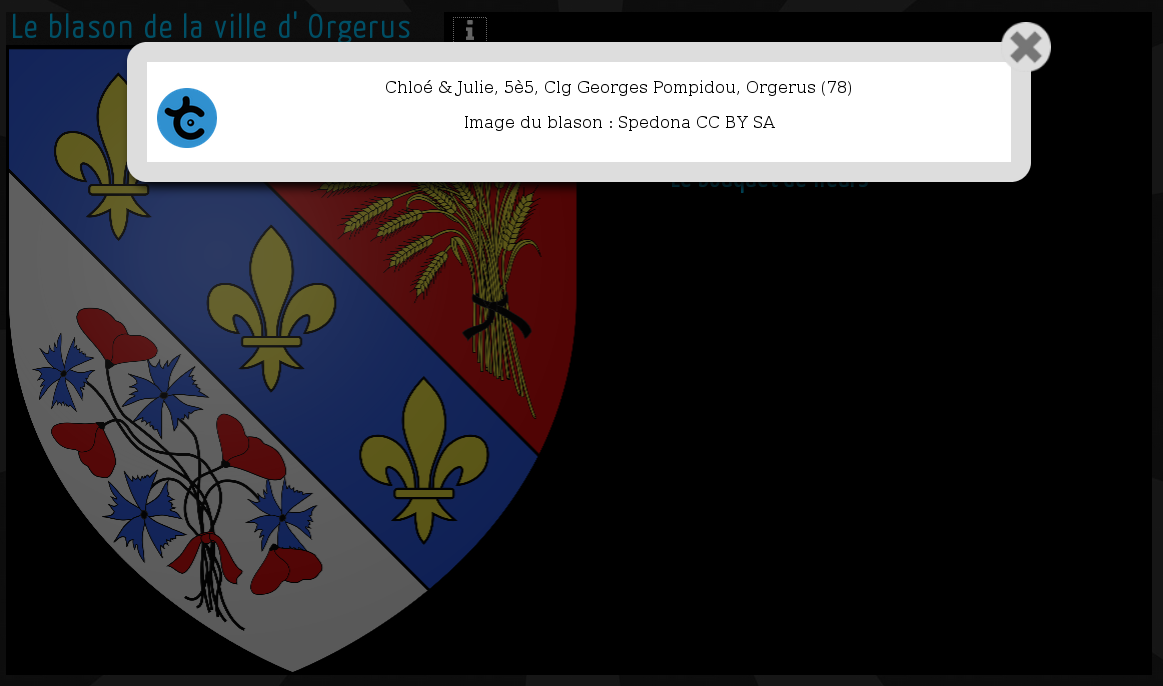
\includegraphics[width=\textwidth]{images/titre_ia}\\
\end{center}

 Le titre renseigné dans les métadonnées du document apparaissent au-dessus
de l'image interactive et donnent son nom à la page web l'affichant. Le
créateur et les droits associés apparaissent dans la pop up accessible via
l'icône «~i~» située à droite du titre de l'image-active.

Vous pouvez sauvegarder votre projet au format svg dès le début du travail,
en allant dans le menu \chemin{Fichier $\rightarrow$ Enregistrer
sous\ldots}.

Vous pouvez, par souci de clarté, supprimer l'extension d'origine de votre
image dans le champ \chemin{Nom} de la fenêtre de dialogue. Enfin, dans le
menu déroulant, choisissez le format de fichier Inkscape svg:

\chemin{SVG Inkscape (*.svg)}.

De nombreux outils d'Inkscape peuvent être utilisés pour détourer les
détails qui deviendront actifs dans l'animation générée par Xia. Parmi
ceux-ci:
\begin{itemize}
 \item 
\includegraphics[scale=0.5]{./images/rec_carre} \chemin{Créer des rectangles et des carrés}
 \item 
\includegraphics[scale=0.5]{./images/cercles} \chemin{Créer des cercles, des ellipses et des arcs}
 \item 
\includegraphics[scale=0.5]{./images/lignes} \chemin{Dessiner des lignes à main levée}
 \item 
\includegraphics[scale=0.5]{./images/bezier} \chemin{Tracer des courbes de
Bézier et des segments de droite}
\end{itemize}

Sans rentrer dans le détail du fonctionnement de ces différents
outils\footnote{Pour cela, lire le
\href{http://inkscape.org/doc/shapes/tutorial-shapes.fr.html}{manuel
d'Inkscape} ou \href{http://en.flossmanuals.net/inkscape/}{le manuel
Floss}.}, sachez que l'outil \chemin{Tracer des courbes de Bézier et des
segments de droite} permet de détourer "clic par clic" (les points de
construction du polygone sont alors appelés des «~nœuds~»). Vous pouvez
refermer votre polygone en cliquant sur le premier nœud de ce même
polygone. Vous pouvez dessiner des \chemin{Courbes de Bézier} en gardant le
clic de votre souris enfoncé après avoir créé un nœud, puis en déplaçant le
curseur pour faire apparaître les poignées de contrôle afin de modifier la
forme de la courbe.


\begin{alerte}
  Si vous laissez une forme ouverte dans Inkscape (une courbe par exemple),
Xia refermera automatiquement celle-ci en joignant son point de départ et
d'arrivée.
\end{alerte}

\begin{alerte}
 L'ordre de création des détails dans Inkscape sera respecté dans l'image
interactive au format html5 (par exemple, le premier détail détouré dans
Inkscape apparaîtra en haut dans le modèle accordéon ou en numéro 1 dans le
modèle boutons). Si vous souhaitez changer cet ordre sans avoir à recréer
tous les détails, lisez la rubrique \ref{couche_XML}.
\end{alerte}

Une fois les détails détourés\footnote{La couleur du contour des détails
dans l'animation générée par Xia sera la même que celle choisie dans
Inkscape.}, vous pouvez les sélectionner avec l'outil \chemin{Sélectionner
et transformer des objets} afin de les redimensionner, les déplacer,
etc.\ldots

\begin{astuce}
Si vous avez des difficultés pour sélectionner un détail que vous avez
détouré, appliquez-lui une couleur de fond. N'importe quelle couleur fera
l'affaire, sauf noir et blanc (pour comprendre pourquoi, lisez la rubrique
\ref{white_black_background}).
\end{astuce}


Vous pouvez accéder aux \chemin{Propriétés de l'objet} par un clic-droit sur
le détail détouré. À partir de là, vous accédez à une fenêtre de dialogue
vous permettant d'ajouter le texte qui sera associé au détail dans l'image
interactive:\\

\begin{center}
 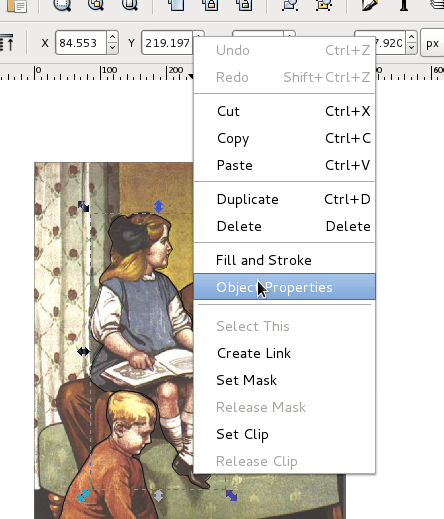
\includegraphics[width=0.5\textwidth]{./images/proprietes_objet}\\ 
\end{center}

Les deux champs devant nécessairement être renseignés dans cette fenêtre
sont les champs \chemin{Titre} et \chemin{Description}. Le titre deviendra
celui du détail, la description son commentaire. N'oubliez pas de cliquer
sur le bouton \chemin{Définir} avant de fermer la fenêtre des
\chemin{Propriétés de l'objet}.

Le processus décrit ci-dessus doit également être effectué avec l'image de
fond: le titre et la description de celle-ci serviront d'introduction
générale à l'image interactive (il s'agit d'un titre et d'un commentaire qui
ne sont pas reliés à un détail particulier).

\subsection{Génération de l'image interactive avec Xia}

Quand tous les détails sont détourés et leurs métadonnées renseignées, Xia
peut être lancé (voir l'illustration \ref{xia_interface}). Vous devez
sélectionner votre fichier svg avec l'icône située en haut à gauche, choisir
la qualité de l'export (voir l'illustration \ref{xia_export_options}), et
enfin choisir un modèle d'export et un répertoire d'enregistrement de
l'image interactive.


En cliquant sur l'une des icônes des modèles d'export, vous générez une
série de fichiers et de répertoires. Ouvrez le fichier \chemin{index.html}
dans un navigateur web pour voir votre image interactive au format html5.

\begin{alerte}
Ce fichier ne peut être séparé des autres pour que l'image-active
fonctionne. Tous les autres fichiers et répertoires générés durant le
processus d'exportation doivent obligatoirement être localisés dans le même
répertoire (voir l'illustration \ref{xia_files}) pour que le fichier
\texttt{index.html} fonctionne correctement. \textbf{Il est donc impératif
de dédier un répertoire spécifique à chaque image-active générée}.
\end{alerte}



\begin{figure}[htp]
\tikzstyle{box}=[draw, text width=4cm, fill=lightgray!50, rounded corners]
\begin{tikzpicture}
  \node[opacity=.5] (bBlue)
{
\includegraphics[scale=.35]{./images/buttonBlue}}; \node[left= .3mm of
bBlue] (aBrown) {
\includegraphics[scale=.35]{./images/audioBrown}};
\node[right= .3mm of bBlue] (guClic)
{
\includegraphics[scale=.35]{./images/game1clic}}; \node[below= .2mm of
bBlue.south, opacity=.5] (pBlue)
{
\includegraphics[scale=.35]{./images/popBlue}}; \node[left= .3mm of pBlue]
(gDDrop) {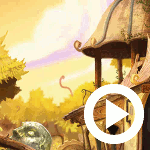
\includegraphics[scale=.35]{./images/gameDragAndDrop}};
\node[right= .3mm of pBlue, opacity=.5] (pYellow)
{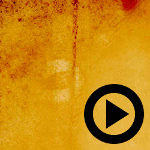
\includegraphics[scale=.35]{./images/popYellow}}; \node[above = .2mm of
guClic.north, opacity=.5] (aCloud)
{
\includegraphics[scale=.35]{./images/accordionCloud}}; \node[above = .2mm
of aCloud.north, opacity=.5] (aBlack)
{
\includegraphics[scale=.35]{./images/accordionBlack}}; \node[left = .3mm of
aBlack] (params) {
\includegraphics[scale=.35]{./images/params}}; \node[left
= .3mm of params] (files) {
\includegraphics[scale=.35]{./images/xia_open}};
\node[left = .3mm of aCloud, opacity=.3] (xialogo)
{
\includegraphics[scale=.47]{./images/xia}};
  
  \node[box, text width=2.5cm,above left = 5mm of files] (filesC) {Sélection
du fichier source svg}; \node[box, above = 5mm of params] (paramsC)
{Sélectionner la qualité de l'export (voir l'illustration
\ref{xia_export_options})}; \node[box,above right = 5mm of aCloud.north
east] (aBlackC)
{\href{http://xia.dane.ac-versailles.fr/demo/tuto/xia1/accordionBlack}{accordionBlack}\\ 
Zone de commentaire large, recommandé pour l'insertion de ressources
multimédias; à utiliser avec des images verticales (portrait)}; \node[box,
right = 5mm of guClic] (aCloudC)
{\href{http://xia.dane.ac-versailles.fr/demo/tuto/xia1/accordionCloud}{accordionCloud}\\ 
Zone de commentaires étroite, laissant davantage de place à l'image en
elle-même ; à utiliser avec des images horizontales (paysage)}; \node[box,
below right = 5mm of pYellow] (pYellowC)
{\href{http://xia.dane.ac-versailles.fr/demo/tuto/xia1/popYellow}{popYellow}\\ 
Pas de zone latérale de commentaire ; un premier clic sur le détail le met
en évidence, et un second fait apparaître le commentaire et enclenche la
fonction zoom}; \node[box, left = 25mm of bBlue] (bBlueC)
{\href{http://xia.dane.ac-versailles.fr/demo/tuto/xia1/buttonBlue}{buttonBlue}\\ 
Pas de zone latérale de commentaire ; les commentaires apparaissent
au-dessus de l'image (recommandé pour les commentaires longs) ; les
utilisateurs accèdent aux commentaires via des boutons situés au-dessus de
l'image interactive}; \node[box, below left = 5mm of pBlue] (pBlueC)
{\href{http://xia.dane.ac-versailles.fr/demo/tuto/xia1/popBlue}{popBlue}\\ 
Pas de zone latérale de commentaire; un premier clic met en évidence le
détail, un second fait apparaître le commentaire (pas de zoom)};
  
  \draw[-stealth] (aBlackC.west) -- (aBlack.north east); \draw[-stealth]
(aCloudC.west) -- (aCloud.south east); \draw[-stealth] (pYellowC.north west)
-- (pYellow.south east); \draw[-stealth] (bBlueC.north east) -- (bBlue.north
west); \draw[-stealth] (pBlueC.north east) -- (pBlue.south west);
\draw[-stealth] (filesC.south east) -- (files.north west); \draw[-stealth]
(paramsC.south) -- (params.north);
  
\end{tikzpicture}
\caption{Les modèles d'export de Xia}
\label{xia_interface}
\end{figure}


\begin{figure}[htp]
\tikzstyle{box}=[draw, text width=4cm, fill=lightgray!50, rounded corners]
\begin{tikzpicture}
  \node (exp_qual) {
\includegraphics[scale=.5]{./images/exp_qual}};
\node[right= .3mm of exp_qual] (exp_firefox)
{
\includegraphics[scale=.5]{./images/exp_firefox}}; \node[below= .2mm of
exp_firefox.south] (exp_1file)
{
\includegraphics[scale=.5]{./images/exp_1file}}; \node[left= .3mm of
exp_1file] (exp_params) {
\includegraphics[scale=.5]{./images/params}};
  
  \node[box, text width=2.5cm, left = 5mm of exp_qual] (exp_qualC)
{Sélectionner la qualité de l'export sur une échelle de 1 à 4}; \node[box,
above right = 5mm of exp_firefox] (exp_firefoxC) {Activer ou désactiver la
création des fichiers pour l'export FirefoxOS (par défaut: désactivé)};
\node[box, right = 5mm of exp_1file] (exp_1fileC) {Dans le cas d'un export
avec fichier unique, vous aurez besoin d'une connexion internet pour accéder
à la ressource. Le moteur de rendu de Xia est hébergé sur les serveurs de
l'académie de Versailles, et est mis à jour automatiquement. Avec cette
configuration, vous ne pouvez pas personnaliser le fond et les icônes (par
défaut: désactivé)};

  \draw[-stealth] (exp_qualC.east) -- (exp_qual.west); \draw[-stealth]
(exp_firefoxC.west) -- (exp_firefox.north east); \draw[-stealth]
(exp_1fileC.west) -- (exp_1file.east);

\end{tikzpicture}
\caption{Les options d'export de Xia}
\label{xia_export_options}
\end{figure}

\begin{figure}[htp]
\tikzstyle{every node}=[draw=black,thick,anchor=west]
\tikzstyle{auto}=[draw=reddebian,fill=reddebian!30, text height=2.5mm]
\tikzstyle{manual}=[draw=bluedane,fill=bluedane!30, text height=2.5mm]
\tikzstyle{manualT}=[fill=bluedane!30,draw=bluedane, rectangle,text
width=5cm, rounded corners]
\tikzstyle{autoT}=[fill=reddebian!30,draw=reddebian, rectangle,text
width=5cm, rounded corners]
\begin{tikzpicture}[grow via three points={one child at (0.5,-0.7) and two children at
(0.5,-0.7) and (0.5,-1.4)}, edge from parent path={(\tikzparentnode.south)
|- (\tikzchildnode.west)}] \node [manual] {mon\_projet/} child { node [auto]
{index.html}}		 child { node [auto] {deploy.html}}		 child { node [auto]
{manifest.webapp}}		 child { node [auto] {css/}} child { node [auto]
{data/}} child { node [auto] {font/}} child { node [auto] {img/}} child {
node [auto] {js/}} child { node [manual] {videos/} child { node [manual]
{video.mp4}} child { node [manual] {video.ogv}} child { node [manual]
{video.webm}} }; \node[manualT] (textM) at (10,-2) {Ces fichiers et
répertoires ont été créés manuellement par le créateur de l'image
interactive. Le répertoire \textcolor{bluedane} {videos} a également été
créé manuellement, dans le but de stocker les vidéos insérées dans les
commentaires de l'image interactive, à l'aide de liens relatifs.};
\node[autoT] (textA) at (10,-6) {Ces fichiers et répertoires sont générés
par Xia durant le processus d'export.}; \draw[-stealth] (textM.west) --
(4,0); \draw[-stealth] (textM.west) -- (5.5,-7); \draw[-stealth]
(textA.west) -- (4,-3);
\end{tikzpicture}
\caption{Fichiers d'une image interactive avec l'export Firefox OS activé}
\label{xia_files}
\end{figure}

En réalité, puisque Xia est également une extension d'Inkscape, vous pouvez
générez vos projets directement depuis ce logiciel: cliquez sur
\chemin{Extensions $\rightarrow$ Divers $\rightarrow$ Xia Édu}, et
choisissez directement la qualité, le modèle d'export, et le répertoire de
destination.

\begin{astuce}
 Si vous utilisez Xia avec GNU/Linux, vous pouvez générer vos animation html5
en utilisant le terminal avec la commande \texttt{xia-converter}. Les
paramètres à utiliser sont \texttt{-i} pour indiquer le fichier en entrée,
\texttt{-o} pour indiquer le répertoire d'export, et \texttt{-t} le template
choisi. Ainsi:\\ \texttt{\$ xia-converter -i monfichier.svg -o
../dossier\_export/ -t accordionBlack}\\ Le template accordionBlack sera
utilisé en cas d'erreur de syntaxe dans la désignation du template
(paramètre \texttt{-t}).
\end{astuce}


\subsection{En résumé}

\begin{enumerate}
 \item Une image interactive est construite dans Inkscape (au format svg). Xia ne
fait que convertir ce fichier source svg en animation html5; 
 \item Le titre de l'image interactive doit être renseigné dans les
\chemin{Métadonnées du document};
 \item Le texte des détails est renseigné dans les \chemin{Propriétés de l'objet},
dans les champs \chemin{Titre} et \chemin{Description};
 \item La description générale de l'image interactive doit être renseignée dans les
\chemin{Propriétés de l'objet} de l'image de fond.
\end{enumerate}

\section{Images interactives enrichies}\label{enriched_IA}

\begin{links}
Visualisez l'\href{http://xia.dane.ac-versailles.fr/demo/tuto/xia2}{image
interactive} créée pour cette partie de la documentation.

Téléchargez le fichier source au format
\href{http://xia.dane.ac-versailles.fr/demo/tuto/xia2/svg/xia2.svg}{svg}.
\end{links}

Dans cette section, l'objectif demeure la création d'une image interactive
«~simple~» (autrement dit, dans laquelle un détail fait apparaître un
commentaire). Cependant, le texte des commentaires sera enrichi par une mise
en forme ou des ressources multimédias.


\newpage
\subsection{Mise en forme du texte}

Afin de mettre en forme le texte, les balises indiquées dans l'illustration
\ref{xia_text_tags} seront utilisées.

\begin{figure}[htp!]
\tikzstyle{descrip}=[font=\sffamily, anchor=north west, text width = 4.3cm]
\tikzstyle{box}=[draw, text width=4cm, fill=lightgray!50, rounded corners,
anchor=north west]
\begin{tikzpicture}
  \node[anchor=north west] (bold)
{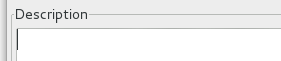
\includegraphics[scale=.5]{./images/Description}}; \node[descrip, below =
-7mm of bold] (boldT) {Ce texte est en ***gras***}; \node[box, right = 3.5cm
of bold] (bolR) {Ce texte est en \textbf{gras}}; \node[anchor=north west,
below = .2cm of bold] (italic)
{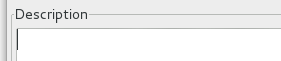
\includegraphics[scale=.5]{./images/Description}}; \node[descrip, below =
-7mm of italic] (italicT) {Ce texte est en **italique**}; \node[box, right =
3.5cm of italic] (italicR) {Ce texte est en \textit{italique}};
\node[anchor=north west, below = .2cm of italic] (texttt)
{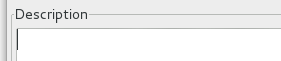
\includegraphics[scale=.5]{./images/Description}}; \node[descrip, below =
-7mm of texttt] (textttT) {Bout de texte \verb!{{{brut}}}!}; \node[box,
right = 3.5cm of texttt] (textttR) {Bout de texte \texttt{brut}};
\node[anchor=north west, below = .2cm of texttt] (link)
{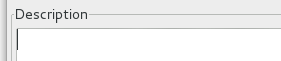
\includegraphics[scale=.5]{./images/Description}}; \node[descrip, below =
7mm of link.north] (linkT) {Un lien vers \verb![https://www.wikipedia.org/]!
\verb![Wikipedia]!}; \node[box, right = 3.5cm of link] (linkR) {Un lien vers
\href{https://www.wikipedia.org/}{Wikipedia}}; \node[anchor=north west,
below = .2cm of link] (relativelinks)
{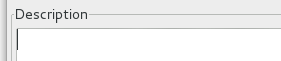
\includegraphics[scale=.5]{./images/Description}}; \node[descrip, below =
-7mm of relativelinks] (relativelinksT) {Un lien vers un
\verb![../dossier/fichier.pdf fichier local]!}; \node[box, right = 3.5cm of
relativelinks] (relativelinksR) {Un lien vers un
\href{/home/geoffrey/ownCloud/DANE/DOSSIERS/XIA/tuto/dossier/fichier.pdf}{fichier
local\footnote{Lien qui ne fonctionnera pas ici!}}}; \node[anchor=north
west, below = .8cm of relativelinks] (bullets)
{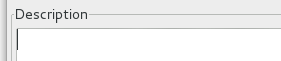
\includegraphics[scale=.5]{./images/Description}}; \node[descrip, below =
-7mm of bullets] (bulletsT) {Faire une liste \\ $\ast$ de puces \\ $\ast$
sur \\ ~$\ast$ 2 niveaux}; \node[box, right = 3.5cm of bullets.south east]
(bulletsR) {Faire une liste \begin{itemize} \item de puces \item sur
\begin{itemize} \item 2 niveaux \end{itemize} \end{itemize} };
\node[anchor=north west, below = 2cm of bullets] (line)
{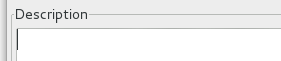
\includegraphics[scale=.5]{./images/Description}}; \node[descrip, below =
7mm of line.north] (lineT) {Tracer \\ - - - - \\ un trait}; \node[box, right
= 3.5cm of line] (lineR) {Tracer \\ \hrulefill \\ un trait};
\end{tikzpicture}
\caption{Balises de mise en forme du texte}
\label{xia_text_tags}
\end{figure}

\subsection{Insérer des ressources multimédias dans les commentaires}\label{enrichissement_multimedia}

L'insertion de ressources multimédias dans les commentaires est chose assez
aisée: copiez-collez l'url de la ressource (qu'elle soit absolue ou
relative) ou le code iframe du service web utilisé pour héberger votre
ressource, et Xia créera automatiquement un lecteur multimédia, pour peu que
celle-ci (image, son, vidéo) fasse partie des formats supportés: 
\begin{description}
 \item[Images] jpg, jpeg, png, gif
 \item [Audio] ogg, mp3
 \item [Video] ogv, webm, mp4
\end{description}

Le lien doit être inséré dans le champ \chemin{Description} des
\chemin{Propriétés de l'objet}:
\begin{description}
 \item[Lien absolu] Si l'url de la ressource est
 
 \verb|http://web.crdp.ac-versailles.fr/02546.ogg|
 

 il suffit alors d'écrire cette url dans le champ \chemin{Description} des
\chemin{Propriétés de l'objet} dans Inkscape.
 
 \item[Lien relatif] Si le fichier de la ressource multimédia se trouve dans le répertoire
d'export de l'image interactive, ou dans un répertoire contenu dans
celui-ci, indiquez simplement le chemin vers le fichier, en considérant le
répertoire d'export comme répertoire racine. Par exemple, si le fichier
\verb|video.ogv| se trouve dans le répertoire  \verb|videos| se trouvant
lui-même dans le répertoire de l'image interactive, indiquez:
 
 \verb|./videos/video.ogv|
 

  pour créer le lecteur. Le \verb|./| signifie que le répertoire \verb|videos|
se trouve dans le répertoire d'exportation. On peut aussi utiliser
\verb|../| pour indiquer que la ressource se trouve dans le répertoire
parent.
\end{description}

Tous les formats vidéos supportés par Xia ne sont cependant pas supportés
nativement par tous les navigateurs web. Il est recommandé d'exporter les
vidéos dans les 3 formats supportés par Xia, et de les déposer dans un seul
et même répertoire (la seule différence entre ces trois vidéos étant donc
leur extension).\\




Ainsi, même si un format particulier est renseigné dans la description (si
l'on suit l'exemple précédent, ce serait \verb|videos/video.ogv|), si le
navigateur web est incapable de lire la ressource, il tentera
automatiquement de lire les fichiers possédant le même nom mais une
extension différente.

La dernière possibilité consiste à insérer un code iframe. Celui-ci sera
interprété et le lecteur du service web apparaîtra, donnant accès à la
ressource.

\subsection{Le modèle «~audioBrown~»: le son à la place du texte}\label{audioBrownsection}

Le modèle «~audioBrown~» est spécifiquement dédié à la création d'images
interactives dans lesquelles les détails sont associés à des sons plutôt
qu'à du texte.

Pour insérer des sons, vous utiliserez des liens absolus ou relatifs en
suivant la méthode décrite dans la section
\ref{enrichissement_multimedia}. Si vous souhaitez que le son soit joué
automatiquement à la sélection du détail, ajoutez la balise \verb|autostart|
après l'url de la ressource \footnote{La balise \texttt{autostart}
fonctionne également avec les autres modèles d'export de Xia.}:\\
\begin{center}
 \verb|sons/son_detail_1.ogg autostart|
\end{center}


\subsection{Insérer des images dans votre image interactive}\label{insertion_images}

Des images au format png peuvent être ajoutées à l'image de fond. Pour faire
cela, sélectionnez \chemin{Fichier $\rightarrow$ Importer} dans Inkscape
afin d'incorporer votre image.

L'image importée n'apparaîtra dans l'animation html5 qu'à une condition: que
vous lui ayez appliqué un fond blanc dans Inkscape. Choisissez la couleur
blanche dans la palette horizontale en bas de l'interface d'Inkscape:\\

\begin{center}
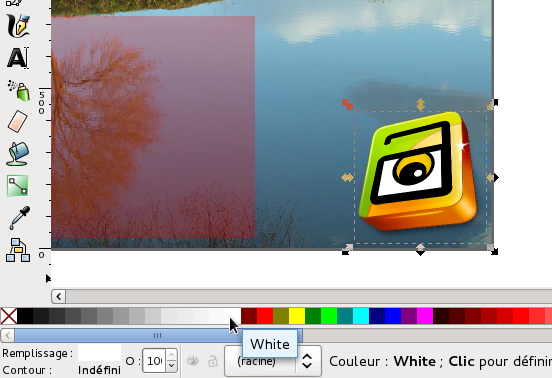
\includegraphics[width=0.6\textwidth]{images/remplissage_blanc}\\ 
\end{center}


En indiquant une url dans le champ \chemin{Titre} des \chemin{Propriétés de
l'objet}, cette image incorporée deviendra un lien cliquable.

\subsection{Faire apparaître une question et dévoiler une réponse}

Vous pouvez créer une icône cliquable, qui empêche temporairement un
utilisateur de lire la suite du commentaire. Vous pouvez même demander à
l'utilisateur d'indiquer un mot de passe pour lire la suite du commentaire.

Pour cela, utilisez dans la description les balises indiquées dans
l'illustration \ref{xia_answer_tags}.

\begin{figure}[htp!]
\tikzstyle{descrip}=[font=\sffamily, anchor=north west, text width = 4.3cm]
\tikzstyle{box}=[draw, text width=4cm, fill=lightgray!50, rounded corners,
anchor=north west]
\begin{tikzpicture}
  \node[anchor=north west] (answer)
{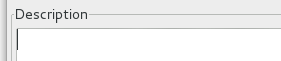
\includegraphics[scale=.5]{./images/Description}}; \node[descrip, below =
-7mm of answer] (answerT) {[[Puis-je vous poser une question? (code=12345):
Bien sûr que c'est possible.]]}; \node[box, right = 3.5cm of answer]
(answerI) {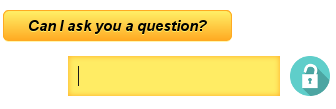
\includegraphics[scale=.5]{./images/answer_code}};
\end{tikzpicture}
\caption{Balises permettant de créer un bouton empêchant temporairement la lecture de
la suite du commentaire.}
\label{xia_answer_tags}
\end{figure}

Utilisez la balise \texttt{[[ (...) ]]} pour indiquer que vous souhaitez
créer une icône, séparez le texte de la question de celui de la réponse avec
la balise \texttt{:}, et ajoutez un code en insérant
\texttt{(code=mot\_de\_passe)} avant la balise \texttt{:}\footnote{Le code
n'est pas obligatoire. Souvenez-vous que vous pouvez utiliser tous les
caractères que vous souhaitez dans le code, sauf le \texttt{)}.}.
  
\subsection{Contrôler le comportement des détails: affichage immédiat et désactivation
du zoom}\label{white_black_background}
\label{couche_XML}

Par défaut, le comportement des détails d'une image interactive est le
suivant:
\begin{itemize}
 \item mise en valeur des détails au survol de la souris ou par un clic sur son
titre dans les commentaires
 \item effet de zoom lors d'un second clic sur le détail actif\footnote{Sauf dans le cas du modèle popBlue.}
\end{itemize}

Ces deux comportements par défaut peuvent être modifiés si vous appliquez un
fond noir ou blanc aux détails détourés (voir la section
\ref{insertion_images} et l'illustration \ref{remplissage_blanc}):
\begin{description}
 \item[Détail avec un fond blanc] Dans l'image interactive, ces détails seront visibles immédiatement, sous la
forme d'un aplat de couleur opaque, cachant l'image de fond; une fois
sélectionné, ce fond sera visible (le zoom demeure actif).
 \item [Détail avec un fond noir] Les utilisateurs devront cliquer pour activer le
détail, mais l'effet de zoom est désactivé.
\end{description}

Conséquence logique: comme un détail ne saurait avoir simultanément un fond
noir et un fond blanc, un détail ne peut donc être à la fois immédiatement
visible et avoir le zoom désactivé.

\subsection{Contrôler l'ordre d'affichage des détails dans la barre latérale des
commentaires}

Par défaut dans une image interactive, les détails apparaissent
verticalement en suivant l'ordre dans lequel ils ont été créés dans Inkscape
(le premier détail créé dans Inkscape correspond à celui placé en haut dans
la barre latérale de l'image interactive).

Pour changer cet ordre par défaut, nous utiliserons l'\chemin{Éditeur XML},
situé dans le menu \chemin{Édition}.

A priori complexe, cette fenêtre de dialogue est en réalité assez simple à
utiliser: en sélectionnant une entrée de l'éditeur XML, le détail
correspondant à celle-ci sera mis en évidence sur l'image. Il ne reste plus 

\begin{center}
 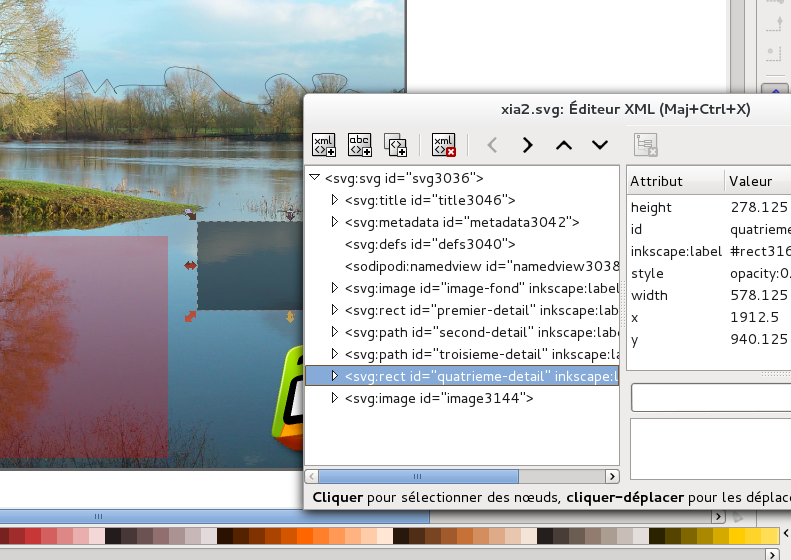
\includegraphics[width=\textwidth]{images/ordre_couches}\\
\end{center}
 
 L'éditeur XML d'Inkscape permet de contrôler l'ordre d'affichage des détails
dans l'image interactive. Remarquez la mise en évidence d'un élément sur
l'image de fond par simple sélection dans l'éditeur.

\subsection{En résumé}

\begin{enumerate}
 \item Vous pouvez enrichir et mettre en forme le texte en utilisant des balises
 \item L'enrichissement multimédia est possible par simple lien (relatif ou absolu)
vers un fichier dont le format est reconnu par Xia
 \item On ajoute des images sur l'image de fond en les incorporant et en leur
appliquant un fond blanc
 \item On peut modifier le comportement par défaut des détails en leur appliquant
une couleur de fond (blanc ou noir)
 \item L'ordre des détails de l'image interactive dépend de l'ordre de leur
création dans Inkscape. Cependant, on peut utiliser l'éditeur XML d'Inkscape
pour modifier cet ordre
\item Il est possible d'empêcher les utilisateurs d'accéder au commentaire en
insérant une icône cliquable et / ou un mot de passe
\end{enumerate}

\newpage

\section{Créer des jeux avec Xia}\label{games_IA}

Jusqu'à maintenant, cette documentation n'a traité que de la création
d'image interactive «~traditionnelle~»: une image de fond, des détails
détourés associés à des commentaires.

Ce type d'image interactive peut être utilisé en classe dans des situations
très variées (les élèves découvrent progressivement une image, ou créent
eux-mêmes une image interactive), mais Xia va plus loin avec de nouvelles
fonctionnalités. On peut désormais créer des jeux, des activités, dans
lesquelles l'utilisateur final a bien davantage à faire que de simplement
cliquer sur des détails et lire du texte.

\begin{figure}[htp]
\tikzstyle{box}=[draw, text width=4cm, fill=lightgray!50, rounded corners]
\begin{tikzpicture}
  \node[opacity=.5] (bBlue)
{
\includegraphics[scale=.35]{./images/buttonBlue}}; \node[left= .3mm of
bBlue] (aBrown) {
\includegraphics[scale=.35]{./images/audioBrown}};
\node[right= .3mm of bBlue] (guClic)
{
\includegraphics[scale=.35]{./images/game1clic}}; \node[below= .2mm of
bBlue.south, opacity=.5] (pBlue)
{
\includegraphics[scale=.35]{./images/popBlue}}; \node[left= .3mm of pBlue]
(gDDrop) {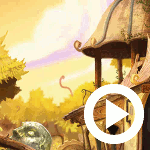
\includegraphics[scale=.35]{./images/gameDragAndDrop}};
\node[right= .3mm of pBlue, opacity=.5] (pYellow)
{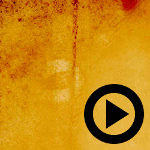
\includegraphics[scale=.35]{./images/popYellow}}; \node[above = .2mm of
guClic.north, opacity=.5] (aCloud)
{
\includegraphics[scale=.35]{./images/accordionCloud}}; \node[above = .2mm
of aCloud.north, opacity=.5] (aBlack)
{
\includegraphics[scale=.35]{./images/accordionBlack}}; \node[left = .3mm of
aBlack] (params) {
\includegraphics[scale=.35]{./images/params}}; \node[left
= .3mm of params] (files) {
\includegraphics[scale=.35]{./images/xia_open}};
\node[left = .3mm of aCloud, opacity=.3] (xialogo)
{
\includegraphics[scale=.47]{./images/xia}};

  
  \node[box, text width=2.5cm,above left = 5mm of files] (filesC) {Sélection
du fichier source au formation svg}; \node[box, above = 5mm of params]
(paramsC) {Sélection de la qualité de l'export}; \node[box, right = 5mm of
guClic] (guClicC)
{\href{http://xia.dane.ac-versailles.fr/demo/tuto/xia3}{game1clic}\\ 
Sélectionner des détails sur une image de fond \\ Tutoriel dans la rubrique
\ref{game1clicsection}}; \node[box, left = 25mm of bBlue] (aBrownC)
{audioBrown template \\ Création d'images interactives dans lesquelles des
détails sont associés à des sons \\ Tutoriel dans la rubrique
\ref{audioBrownsection}}; \node[box, below left = 5mm of pBlue] (gDDropC)
{\href{http://xia.dane.ac-versailles.fr/demo/tuto/xia5}{gameDragAndDrop}\\ 
Glisser et déposer des éléments sur l'image de fond \\ Tutoriel dans la
rubrique \ref{gameDragAndDropsection}};
  
  \draw[-stealth] (guClicC.west) -- (guClic.east); \draw[-stealth]
(gDDropC.north) -- (gDDrop.south); \draw[-stealth] (aBrownC.north east) --
(aBrown.north); \draw[-stealth] (filesC.south east) -- (files.north west);
\draw[-stealth] (paramsC.south) -- (params.north);
  
\end{tikzpicture}
\caption{Les modèles multimédias et ludiques de Xia}
\label{xia_interface2}
\end{figure}

\subsection{Premier principe ludique: sélectionner, trouver des éléments dans une image}\label{game1clicsection}

\textit{Le principe ludique décrit dans cette partie de la documentation est
le suivant: le joueur doit sélectionner des détails dans une image, quand il
a sélectionné les éléments indiqués dans la consigne, un message de fin
apparaît.}


\begin{links}
Visualisez l'\href{http://xia.dane.ac-versailles.fr/demo/tuto/xia3}{image
interactive} créée pour cette partie de la documentation.

Téléchargez le fichier source au format
\href{http://xia.dane.ac-versailles.fr/demo/tuto/xia3/svg/xia3.svg}{svg}.
\end{links}

Ce type de jeu est presque le type d'image interactive la plus facile à
créer. Vous devez uniquement détourer les détails que le joueur devra
sélectionner. 

Les consignes doivent être indiquées dans les métadonnées du document. Xia
cherchera les informations relatives aux consignes dans le champ
\chemin{Description} des métadonnées du document (voir la section
\ref{preparation_svg}: \chemin{Fichier $\rightarrow$ Métadonnées du
document}), et créera une pop up affichant ces consignes à l'ouverture du
jeu. Le joueur pourra les lire, fermer la fenêtre puis jouer.

Quand un joueur termine le jeu, un message apparaît automatiquement. Le
score nécessaire pour le déclenchement de ce message et le message en
lui-même doivent être renseignés à l'intérieur de balises
\texttt{<score></score>}\footnote{Il faut indiquer un nombre. Ce nombre n'a
pas à être similaire au nombre de détails se trouvant sur l'image.} et
\texttt{<message></message>} dans le champ \chemin{Description} des
\chemin{Propriétés de l'objet} de l'image de fond\footnote{En créant une
image interactive traditionnelle, ce champ crée l'introduction de
l'animation, non reliée à un détail particulier.}. 

Vous trouverez tous les détails sur l'endroit et la manière d'indiquer ces
informations dans le tableau \ref{tag1_sumup}.

\begin{table}
 \begin{tabular}{|l|p{2in}|p{2in}|}
 \hline
  Objectif & Renseigner le nombre de réponses correctes permettant de terminer le jeu & Afficher un message\\
  \hline
  Balise & \texttt{<score></score>}| & \texttt{<message></message>}\\
  \hline
  Exemple & \multicolumn{2}{|l|}{\texttt{<score>6</score>}}\\
   & \multicolumn{2}{|l|}{\texttt{<message>Bravo!}}\\
    & \multicolumn{2}{|l|}{\texttt{Vous avez terminé le jeu!</message>}}\\
  \hline
 \end{tabular}
\caption{Résumé des balises du jeu game1clic}
\label{tag1_sumup}
\end{table}
 
\begin{astuce}
Le texte inséré dans la balise \verb|<message></message>| peut être enrichi
avec des images, des vidéos, du son. On peut aussi imaginer ajouter un lien
vers un autre jeu, ce qui permettrait aux utilisateurs d'enchaîner les jeux
par degré de difficulté.
\end{astuce}

\begin{wrapfigure}{r}{45mm}
  \centering
  
\includegraphics[scale=0.7]{./images/game1clic} 
\end{wrapfigure}

Choisir le modèle d'export \chemin{game1clic} pour générer l'image
interactive.


\subsubsection{\emph{Astuces pour la création d'image interactive «~avancée~»\ldots}
Montrer la progression du joueur}

Il est possible de faire s'afficher des éléments graphiques quand le joueur
sélectionne une réponse correcte. Ces éléments peuvent être des png importés
ou des formes directement dessinées dans Inkscape. Comme Xia considère
qu'une forme dessinée avec les outils d'Inkscape est un détail, il faudra
transformer ces formes en utilisant l'outil «~copie bitmap~». Par exemple:
\begin{enumerate}
 \item Dessinez une étoile aux bords jaunes et au fond jaune avec les outils de
dessin d'Inkscape 
 \item Sélectionnez cette étoile, et cliquez sur \chemin{Édition $\rightarrow$
Créer une copie bitmap}
 \item Supprimer l'étoile créée avec les outils de dessin
\end{enumerate}

Une fois les éléments importés (format png) ou créés (copie bitmap des
formes dessinées manuellement), appliquez-leurs les caractéristiques
suivantes:
\begin{center}
\chemin{Interactivité > OnClick} = \verb|off|
\end{center}
Ensuite, groupez le détail cliquable et son élément graphique (en cliquant
successivement sur le détail et l'élément en maintenant la touche \Shift
enfoncée), puis en sélectionnant \chemin{Grouper} dans le menu
\chemin{Objet} d'Inkscape.

\subsubsection{\emph{Astuces pour la création d'image interactive «~avancée~»\ldots} Mettre
en évidence les erreurs du joueur}

On voit clairement l'intérêt pédagogique des jeux basés sur le principe de
la sélection\ldots mais on voit également rapidement comment des élèves
peuvent être tentés de contourner le dispositif ludique pour terminer les
jeux sans avoir à réfléchir (par exemple, en cliquant frénétiquement partout
sur l'image, jusqu'à trouver par hasard tous les détails répondant à la
consigne).

C'est la raison pour laquelle il peut être intéressant de mettre en valeur
les erreurs commises par le joueur.

Pour cela, il faudra prévoir les erreurs pouvant être commises, et placer
sur l'image des éléments graphiques symbolisant l'erreur (croix rouge,
etc.). Ces éléments pouvant être des images au format png importées ou des
formes dessinées dans Inkscape, puis copiées en bitmap. Ces éléments devront
posséder les caractéristiques suivantes:
\begin{center}
\chemin{Interactivité > OnClick} = \verb|disable-score| 
\end{center}
Une fois la balise \verb|disable-score| appliquée, le détail demeure
cliquable, mais sa sélection n'ajoutera pas un point au compteur surveillant
le score pour délivrer le message de fin.

\subsubsection{\emph{Astuces pour la création d'image interactive «~avancée~»\ldots} Deux
compteurs de score}

En indiquant \verb|score2| dans le champ \chemin{onclick}
(\chemin{Propriétés de l'objet $\rightarrow$ Interactivité}) du détail, et
en utilisant les balises\\
\texttt{<score2></score2>} et \texttt{<message2></message2>} dans les
\chemin{Propriétés de l'objet} de l'image de fond, on peut créer un système
de double comptage des points, dans lequel l'utilisateur peut sélectionner
deux types de détails différents.

Ainsi, vous pouvez créer un jeu où 3 détails comportent la balise
\texttt{score2} (cette balise correspondant à des erreurs), et indiquez dans
les \chemin{Propriétés de l'objet} de l'image de fond:\\ 
\texttt{<score>4</score>\\ <message>Bravo!</message>\\ <score2>3</score2>\\ 
<message2>3 erreurs... Ça fait beaucoup...\\
Concentrez-vous et recommencez!...</message2>}\\


\subsection{Second principe ludique: classer, organiser, hiérarchiser}\label{gameDragAndDropsection}

Le second type de jeu pouvant être créé avec Xia est basé sur le principe du
glisser-déposer. Des étiquettes déplaçables sont déposées sur l'image de
fond. Quand tous les éléments ont été placés sur leur zone de dépôt, un
message apparaît, annonçant la fin du jeu.

\begin{links}
Visualisez l'\href{http://xia.dane.ac-versailles.fr/demo/tuto/xia5}{image
interactive} créée pour cette partie de la documentation.

Téléchargez le fichier source au format
\href{http://xia.dane.ac-versailles.fr/demo/tuto/xia5/svg/xia5.svg}{svg}.
\end{links}

Voici comment créer un jeu basé sur le principe du glisser-déposer:
\begin{enumerate}
 \item Dans Inkscape:
\begin{itemize}
 \item Choisir une image de fond
 \item Créer les éléments que les utilisateurs de votre image interactive auront à
déplacer et à déposer (autrement dit: des images, des mots ou groupes de
mots)
 \item Créer la fenêtre surgissante de consignes en éditant les informations du
champ \chemin{Fichier $\rightarrow$ Métadonnées du document $\rightarrow$
Description}\footnote{Exactement comme dans le jeu game1clic}
 \item En renseignant les métadonnées, faites correspondre chaque élément à une
zone de dépôt (ces zones de dépôts étant en réalité des détails détourés)
\end{itemize}
 \item Dans Xia
 \begin{itemize}
  \item Exporter le fichier source au format svg avec le modèle «~gameDragAndDrop~»
 \end{itemize}
\end{enumerate}

Deux méthodes peuvent être utilisées pour créer les éléments que les joueurs
auront à glisser et déposer. La première, très simple, consiste à utiliser
un utilitaire de capture d'écran capable de créer des petites images au
format png, puis d'importer celles-ci dans Inkscape. Il est également
possible de créer ces éléments directement dans Inkscape. Par exemple, en
créant un texte, en regroupant ce texte avec une forme puis en faisant une
copie bitmap de cet ensemble. Les éléments à déplacer doivent être associés
à leur zone de dépôt \footnote{\textbf{Un} objet ne pouvant être associé
qu'à \textbf{une} zone de dépôt.}.

Vous trouverez dans le tableau \ref{tag2_sumup} un résumé des balises à
renseigner dans les \chemin{Propriétés de l'objet} des éléments à déplacer
et des zones de dépôts afin de les faire correspondre les unes aux autres.

\begin{table}
\begin{tabular}{|p{1.in}|p{2.5in}|p{1.5in}|}
\hline
 & Élément à déplacer (objets à glisser et déposer) & Détail détouré (zone de dépôt)\\
\hline
Champ ID & & \verb|Titre_du_détail|\\
\hline
Champ description & \verb|<target>Titre_du_détail</target>| & \\
\hline
\end{tabular}
\caption{Résumé des balises à utiliser dans le jeu gameDragAndDrop}
\label{tag2_sumup}
\end{table}

\begin{wrapfigure}{r}{45mm}
  \centering
  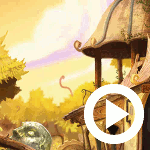
\includegraphics[scale=0.7]{./images/gameDragAndDrop} 
\end{wrapfigure}


Il faut donc «~jumeler~» les éléments à glisser-déposer avec leur zone de
dépôt en faisant correspondre le champ \chemin{ID} de la zone de dépôt au
champ \chemin{Description} de l'élément à glisser déposer. La seule
subtilité tient dans la balise \verb|<target></target>| devant être indiquée
dans la \chemin{Description}.

Choisissez le modèle \chemin{gameDragAndDrop} pour générer l'image
interactive.



\subsubsection{Comment ajouter un effet «~aimant~» dans le jeu gameDragAndDrop}

Si vous indiquez \verb|<magnet>on</magnet>| dans le champ
\chemin{Description} de la zone de dépôt, un effet aimant sera activé quand
le joueur déposera l'élément sur celle-ci.

\subsubsection{Deux façons de donner des indices aux joueurs: les infobulles et les liens
sur les zones de dépôt}

Il est possible de faire s'afficher des infobulles lorsque la souris survole
certains détails. Pour cela, créez l'infobulle avec une image au format png
importée ou une copie bitmap d'un texte créé dans Inkscape\footnote{Ou une
copie bitmap d'une forme groupée avec du texte\ldots}, et appliquez à cette
infobulle une \chemin{ID} spéicifique dans les \chemin{Propriétés de
l'objet}. Ensuite, indiquez la balise
\verb|<tooltip>ID_de_l_infobulle</tooltip>| dans le champ
\chemin{Description} des \chemin{Propriétés de l'objet} du détail censé
déclencher l'apparition de l'infobulle (par exemple, dans l'image
ci-dessous: au survol de la souris, le carré jaune fait apparaître
l'infobulle "Test"):\\


\begin{center}
 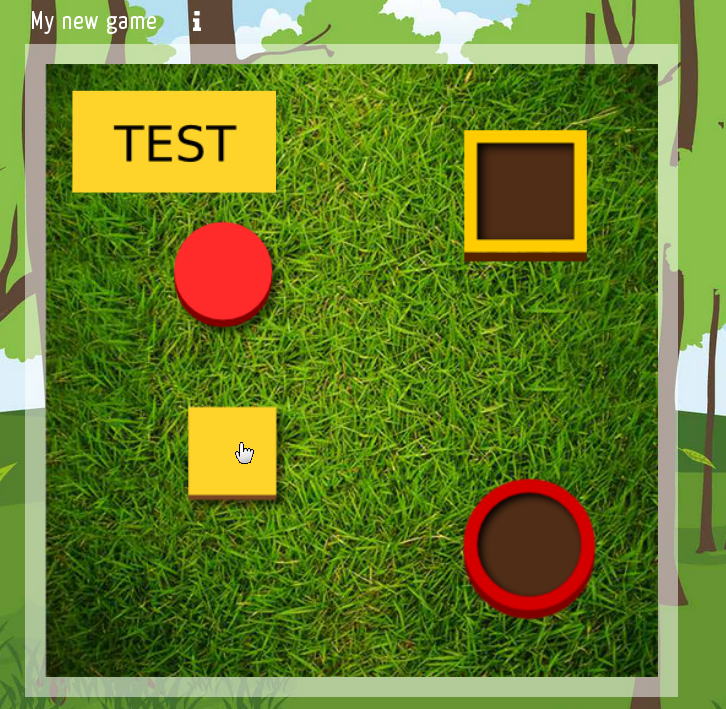
\includegraphics[width=0.5\textwidth]{images/tooltip_example}\\
 \end{center}


Notez que cette fonctionnalité est également disponible dans le jeu
game1clic.
 
Une autre méthode consiste à insérer un lien dans le champ \chemin{Titre}
des \chemin{Propriétés de l'objet} de la zone de dépôt. L'utilisateur peut
cliquer sur cette zone ou y déposer l'étiquette correspondante pour suivre
le lien.

\subsection{Troisième principe ludique: les collisions}

\textit{Le principe ludique documenté dans cette section est le suivant: le
joueur doit déplacer des éléments vers des zones de dépôt, mais les
déplacements de ces éléments ne peuvent avoir lieu que dans certaines
limites. Le jeu de type «~collisions~» peut ainsi être utilisé pour créer
des labyrinthes, des taquins.}

Pour créer ce type de jeu, ajoutez la balise
\verb|<collisions>on</collisions>| à l'image de fond. Une fois cela fait,
tous les détails deviennent «~solides~», et bloquent le déplacement des
objets qu'il faut déplacer (images au format png importées, ou copie bitmap
de formes dessinées avec Inkscape).

Le jeu de type «~collisions~» est en réalité un jeu de type gameDragAndDrop,
puisque la résolution passe par le dépôt d'un ou plusieurs éléments à
certains endroits de l'image. Les balises nécessaires dans ce type de jeu
sont donc les mêmes que dans le jeu gameDragAndDrop
\footnote{\texttt{<target></target>} sur les objets,
\texttt{<score></score>} sur l'image de fond: voir la section
\ref{gameDragAndDropsection}.}, mais il faudra penser à appliquer la balise
\verb|<collisions>off</collisions>| sur les zones de dépôts, dans le champ
\chemin{Description}.
\newpage
\subsection{En résumé}

Ces tableaux résument les balises pouvant être utilisées dans le cadre de la
création de jeux avec Xia:

\begin{table}[thp]
 \begin{tabular}{|p{.5cm}|p{2cm}|p{10cm}|}
 \hline
 \multicolumn{3}{|l|}{Modèle \chemin{game1clic}} \\
 \hline
 \multicolumn{3}{|l|}{\texttt{<score></score>}}\\
 \hline
 & \emph{Rôle} & Permet de régler le nombre de bonnes réponses nécessaires pour faire
apparaître le message de fin du jeu\\
 & \emph{Élément}  & Image de fond \\
 & \emph{Où?} & \chemin{Propriétés de l'objet $\rightarrow$ Description} \\
 & \emph{Quoi?} & Le nombre de bonnes réponses nécessaires à la résolution du jeu\\
 \hline
 \multicolumn{3}{|l|}{\texttt{<message></message>} }\\
 \hline
  & \emph{Rôle} & Fait apparaître le message de fin du jeu \\
  & \emph{Élément}  & Image de fond \\
  & \emph{Où?} & \chemin{Propriétés de l'objet $\rightarrow$ Description}\\ 
  & \emph{Quoi?} & Un message que vous pouvez si nécessaire enrichir avec des ressources
multimédias ou un lien hypertexte\\
  \hline
  \multicolumn{3}{|l|}{\texttt{off}}\\
  \hline
  & \emph{Rôle} & Rend un détail insensible au clic \\
  & \emph{Élément} & Détail \\
  & \emph{Où?} & \chemin{Propriétés de l'objet $\rightarrow$ Interactivité $\rightarrow$
Onclick}\\
 \hline
  \multicolumn{3}{|l|}{\texttt{disable-score}}\\
  \hline
  & \emph{Rôle} & Rend un détail détouré cliquable, mais sa sélection n'ajoutera pas de point
au compteur de score \\
  & \emph{Élément} & Détail \\
  & \emph{Où?} & \chemin{Propriétés de l'objet $\rightarrow$ Interactivité $\rightarrow$
Onclick}\\
  \hline
    \multicolumn{3}{|l|}{\texttt{score2}}\\
  \hline
  & \emph{Rôle} & Ajoute un point au deuxième compteur de score \\
  & \emph{Élément} & Détail \\
  & \emph{Où?} & \chemin{Propriétés de l'objet $\rightarrow$ Interactivité $\rightarrow$
Onclick}\\
  \hline
  \multicolumn{3}{|l|}{\texttt{<tooltip></tooltip>}}\\
  \hline
  & \emph{Rôle} & Affiche une infobulle au survol de la souris \\
  & \emph{Élément} & Détail \\
  & \emph{Quoi?} & Assurez-vous que ce champ est identique à l'ID de l'élément servant
d'infobulle\\
  & \emph{Où?} & \chemin{Propriétés de l'objet $\rightarrow$ Description}\\
  \hline
 \multicolumn{3}{|l|}{\texttt{<score></score>}}\\
 \hline
 & \emph{Rôle} & Permet de régler le nombre de bonnes réponses nécessaires pour faire
apparaître le message de fin du jeu\\
 & \emph{Élément}  & Image de fond \\
 & \emph{Où?} & \chemin{Propriétés de l'objet $\rightarrow$ Description} \\
 & \emph{Quoi?} & Le nombre de bonnes réponses nécessaires à la résolution du jeu\\
 \hline
 \multicolumn{3}{|l|}{\texttt{<message2></message2>}}\\
 \hline
  & \emph{Rôle} & Fait apparaître le second message de fin du jeu, dans le cas d'un jeu à
double score \\
  & \emph{Élément}  & Image de fond \\
  & \emph{Où?} & \chemin{Propriétés de l'objet $\rightarrow$ Description}\\ 
  & \emph{Quoi?} & Un message que vous pouvez si nécessaire enrichir avec des ressources
multimédias ou un lien hypertexte\\
  \hline
  \end{tabular}
  \caption{Balises à insérer pour un jeu de type game1clic}
 \end{table}
 
 \begin{table}[thp]
 \begin{tabular}{|p{.5cm}|p{2cm}|p{10cm}|}
 \hline
 \multicolumn{3}{|l|}{Modèle \chemin{gameDragAndDrop}} \\
 \hline
 \multicolumn{3}{|l|}{\texttt{<score></score>}}\\
 \hline
 & \emph{Rôle} & Permet de régler le nombre de bonnes réponses nécessaires pour faire
apparaître le message de fin du jeu\\
 & \emph{Élément}  & Image de fond \\
 & \emph{Où?} & \chemin{Propriétés de l'objet $\rightarrow$ Description} \\
 & \emph{Quoi?} & Le nombre de bonnes réponses nécessaires à la résolution du jeu\\
 \hline
 \multicolumn{3}{|l|}{\texttt{<message></message>} }\\
 \hline
  & \emph{Rôle} & Fait apparaître le message de fin du jeu \\
  & \emph{Élément}  & Image de fond \\
  & \emph{Où?} & \chemin{Propriétés de l'objet $\rightarrow$ Description}\\ 
  & \emph{Quoi?} & Un message que vous pouvez si nécessaire enrichir avec des ressources
multimédias ou un lien hypertexte\\
  \hline
  \multicolumn{3}{|l|}{\texttt{<target></target>}}\\
  \hline
  & \emph{Rôle} & Indique la correspondance entre l'élément à déplacer et la zone de dépôt \\
  & \emph{Élément} & Élément à déplacer \\
  & \emph{Où?} & \chemin{Propriétés de l'objet $\rightarrow$ Description}\\
  & \emph{Quoi?} & Assurez-vous que ce champ est identique à l'ID de la zone de dépôt\\
  \hline
  \multicolumn{3}{|l|}{\texttt{<magnet>on</magnet>}}\\
  \hline
  & \emph{Rôle} & Ajoute un effet «~aimant~» \\
  & \emph{Élément} & Zone de dépôt \\
  & \emph{Où?} & \chemin{Propriétés de l'objet $\rightarrow$ Description} \\
  \hline
  \multicolumn{3}{|l|}{\texttt{<collisions>on</collisions>}}\\
  \hline
  & \emph{Rôle} & Active le jeu de type "collisions" \\
  & \emph{Élément} & Image de fond \\
  & \emph{Où?} & \chemin{Propriétés de l'objet $\rightarrow$ Description} \\
  \hline
  \multicolumn{3}{|l|}{\texttt{<collisions>off</collisions>}}\\
  \hline
  & \emph{Rôle} & Crée une zone de dépôt dans un jeu de type "collisions"\\
  & \emph{Élément} & Zone de dépôt\\
  & \emph{Où?} & \chemin{Propriétés de l'objet $\rightarrow$ Description} \\
  \hline
    \multicolumn{3}{|l|}{\texttt{<tooltip></tooltip>}}\\
  \hline
  & \emph{Rôle} & Affiche une infobulle au survol de la souris \\
  & \emph{Élément} & Zone de dépôt, éléments à déplacer \\
  & \emph{Quoi?} & Assurez-vous que ce champ est identique à l'ID de l'élément servant
d'infobulle\\
  & \emph{Où?} & \chemin{Propriétés de l'objet $\rightarrow$ Description}\\
  \hline
  \end{tabular}
  \caption{Balises à insérer en vue d'un export gameDragAndDrop}
\end{table} 

\listoffigures \listoftables

\end{document}
